%% Copernicus Publications - AGILE-GISS Template (version 2023) for LaTeX Manuscript Preparation
%% CascadeCBF Shortpaper

%% 2-column AGILE papers
\documentclass[agile, final]{copernicus-agile}

\usepackage{fontawesome5}
\usepackage{enumitem}
\usepackage{algorithm}
\usepackage{algorithmic}
\usepackage{amsmath}
\usepackage{tikz}
\usetikzlibrary{shapes.multipart,positioning,arrows.meta,decorations.pathreplacing}

\hypersetup{
    colorlinks=true,
    filecolor=magenta,
    urlcolor=blue,
    linkcolor=blue,
    citecolor=black,
}

% Math operators for algorithms
\DeclareMathOperator{\val}{\textbf{val}}
\DeclareMathOperator{\hashfn}{\textbf{hash}}

\begin{document}

\title{CascadeCBF: Probabilistic Counting for Sparse Spatial Point Clouds}

\Author[1]{Moritz}{Laass}
\Author[1]{Martin}{Werner\orcid{0000-0002-4095-6665}}

\affil[1]{Technical University of Munich, TUM School of Engineering and Design, Munich, Germany}

\correspondence{Moritz Laass (\color{blue}moritz.laass@tum.de)}

\firstpage{1}

\maketitle

\begin{abstract}
Spatial point datasets often exhibit power-law frequency distributions where few locations receive most observations. Traditional counting bloom filters struggle with such distributions due to fixed counter bit-depths. We present CascadeCBF, a multi-layer probabilistic data structure using cascading overflow: counters in lower layers handle infrequent locations, while overflow cascades to higher layers for hotspots. CascadeCBF supports spatial operations (union, intersection, aggregation) directly on the compressed representation. Evaluation on Zipfian distributions shows CascadeCBF with minimal increment and independent hashes matches the memory efficiency of Spectral Bloom Filters and Count-Min Sketch, while the multi-layer design enables exact counts for highly skewed data.

\textbf{Submission Type.} Short Paper \quad \textbf{BoK Concepts.} [AM] Analytical Methods, [DM] Data Modeling

\keywords{probabilistic data structures, counting bloom filter, spatial data, cardinality estimation}

\end{abstract}

%% =============================================================================
%% INTRODUCTION
%% =============================================================================
\introduction
\label{sec:intro}

Geospatial applications generate point data at massive scales---billions of geotagged posts, GPS traces, and sensor observations. A key operation is \emph{cardinality estimation}: counting observations per location for hotspot detection, trajectory analysis, and spatial aggregation. Probabilistic structures like Counting Bloom Filters (CBFs)~\cite{bloom_space/time_1970} offer space-efficient frequency estimation, but fixed bit-depth counters either overflow at hotspots or waste memory on rare locations. This is problematic for spatial data, which typically follows power-law distributions: a few locations (city centers, popular venues) receive orders of magnitude more observations than the majority.

We introduce \emph{CascadeCBF}, extending GloBiMaps~\cite{werner2019globimaps} with cascading overflow: layers use increasing bit-depths, and increments cascade upward when counters saturate. Our contributions: (1) an overflow bit protocol for efficient multi-layer counting with cache-friendly access patterns; (2) spatial operations (union, intersection, aggregation) directly on compressed representations; (3) comprehensive evaluation on synthetic and real-world datasets showing competitive accuracy and throughput.


%% =============================================================================
%% BACKGROUND
%% =============================================================================
\section{Background}
\label{sec:background}

\subsection{Bloom Filter Theory}

A Bloom filter~\cite{bloom_space/time_1970} represents a set using an $m$-bit array and $k$ hash functions. Inserting element $e$ sets bits at positions $h_1(e), \ldots, h_k(e)$; membership queries check if all $k$ positions contain ones. The \emph{fraction of zeros} after inserting $n$ elements is:
\begin{equation}
\text{foz} = \left(1 - \frac{1}{m}\right)^{kn} \approx e^{-kn/m}
\end{equation}
The false positive probability---finding $k$ ones at random positions---is $p = (1 - \text{foz})^k$. Minimizing $p$ yields the optimal number of hash functions: $k^* = (m/n) \ln 2 \approx 0.693(m/n)$.

\subsection{Counting Extensions}

Counting Bloom Filters (CBFs)~\cite{fan2000summary} replace single bits with $b$-bit counters, enabling frequency queries and deletions. However, fixed bit-depth creates a tradeoff: small counters overflow on hotspots while large counters waste memory on rare items. Spectral Bloom Filters~\cite{cohen2003spectral} improve accuracy via \emph{minimal increment} (MI)---only incrementing counters at the current minimum count. Count-Min Sketch~\cite{cormode2005improved} provides provable error bounds: estimates exceed true counts by at most $\varepsilon N$ with probability $1-\delta$, requiring $k = \lceil \ln(1/\delta) \rceil$ rows.

Multi-layer approaches address the bit-depth tradeoff. Dynamic Count Filters~\cite{aguilar-saborit_dynamic_2006} resize counters dynamically but incur rebuild overhead. Multilayer Compressed CBFs~\cite{ficara_multilayer_2008} use Huffman coding for variable-length counters. Real-world spatial data follows power-law (Zipfian) distributions~\cite{broder2004network}: a few locations receive most observations, making fixed-depth counters particularly inefficient.

GloBiMaps~\cite{werner2019globimaps} adapt Bloom filters for sparse spatial rasters by hashing discretized coordinates, supporting set operations (union, intersection) directly on the compressed representation.


%% =============================================================================
%% CASCADECBF
%% =============================================================================
\section{CascadeCBF}
\label{sec:cgm}

\begin{figure}[ht]
\centering
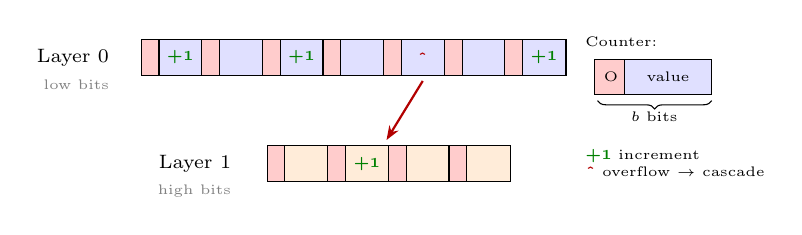
\begin{tikzpicture}[
    counter/.style={draw, minimum width=0.55cm, minimum height=0.45cm, font=\tiny},
    obit/.style={draw, fill=red!20, minimum width=0.22cm, minimum height=0.45cm, font=\tiny},
    vbits/.style={draw, fill=blue!12, minimum width=0.55cm, minimum height=0.45cm, font=\tiny},
    arr/.style={-{Stealth[length=1.8mm]}, thick}
]
% Layer 0 - base layer (wide) - holds LOW bits
\node[font=\scriptsize, anchor=east] at (-3.2,1.6) {Layer 0};
\node[font=\tiny, gray, anchor=east] at (-3.2,1.25) {low bits};

\foreach \i in {0,1,2,3,4,5,6} {
    \pgfmathsetmacro{\x}{-2.8+\i*0.77}
    \node[obit] at (\x,1.6) {};
    \node[vbits] at (\x+0.385,1.6) {};
}
% Labels for +1 and overflow
\node[font=\tiny, green!50!black] at (-2.42,1.6) {\textbf{+1}};
\node[font=\tiny, green!50!black] at (-0.88,1.6) {\textbf{+1}};
\node[font=\tiny, red!70!black] at (0.66,1.6) {\textbf{\^{}}};
\node[font=\tiny, green!50!black] at (2.2,1.6) {\textbf{+1}};

% Cascade arrow from overflowed counter
\draw[arr, red!70!black] (0.66,1.3) -- (0.2,0.55) node[midway, right, font=\tiny] {};

% Layer 1 - overflow layer (narrower) - holds HIGH bits
\node[font=\scriptsize, anchor=east] at (-1.65,0.25) {Layer 1};
\node[font=\tiny, gray, anchor=east] at (-1.65,-0.1) {high bits};

\foreach \i in {0,1,2,3} {
    \pgfmathsetmacro{\x}{-1.2+\i*0.77}
    \node[obit] at (\x,0.25) {};
    \node[vbits, fill=orange!15] at (\x+0.385,0.25) {};
}
\node[font=\tiny, green!50!black] at (-0.05,0.25) {\textbf{+1}};

% Counter structure legend (right side)
\node[font=\tiny, anchor=west] at (2.6,1.8) {Counter:};
\node[obit, minimum width=0.35cm] (lo) at (3.05,1.35) {\tiny O};
\node[vbits, minimum width=1.1cm] at (3.775,1.35) {\tiny value};
\draw[decorate, decoration={brace, amplitude=3pt, mirror}] (2.88,1.05) -- (4.33,1.05);
\node[font=\tiny] at (3.6,0.85) {$b$ bits};

% Legend
\node[font=\tiny, anchor=north west, align=left] at (2.6,0.55) {
\textcolor{green!50!black}{\textbf{+1}} increment\\
\textcolor{red!70!black}{\textbf{\^{}}} overflow $\to$ cascade
};

\end{tikzpicture}
\caption{CascadeCBF: Layer 0 holds low-order bits; when value bits saturate (\^{}), overflow bit O is set and Layer 1 (high-order bits) is incremented.}
\label{fig:architecture}
\end{figure}

CascadeCBF consists of $k$ hash functions and layers $L_0, \ldots, L_{\Lambda-1}$ with increasing bit-depths $b_0 < \cdots < b_{\Lambda-1}$. The \emph{overflow bit protocol} (Fig.~\ref{fig:architecture}) reserves each counter's high bit as overflow flag: when value bits saturate, the flag is set and increments cascade to the next layer. Since Layer 1 is only accessed every $2^{b_0-1}$ increments, most operations touch only Layer 0---improving cache locality.

We use the \emph{hashing trick}: a single MurmurHash3 call produces two 64-bit values $(h_1, h_2)$, from which $k$ hash positions are derived as $j_i = (h_1 + (i+1) \cdot h_2) \bmod m_x$.

\begin{algorithm}[ht]
\caption{PUT Operation}
\label{alg:put}
\begin{algorithmic}[1]
\REQUIRE CascadeCBF $A$, point $p$
\STATE $h_1, h_2 \gets \hashfn(p)$
\FOR{$i = 0$ \TO $k-1$}
  \FOR{$x = 0$ \TO $\Lambda-1$}
    \STATE $j \gets (h_1 + (i+1) \cdot h_2) \bmod m_x$
    \IF{overflow bit at $\val(j, L_x)$ not set}
      \STATE increment $\val(j, L_x)$
      \STATE \textbf{break} \COMMENT{move to next hash function}
    \ENDIF
  \ENDFOR
\ENDFOR
\end{algorithmic}
\end{algorithm}

\begin{algorithm}[ht]
\caption{GET Operation}
\label{alg:get}
\begin{algorithmic}[1]
\REQUIRE CascadeCBF $A$, point $p$
\ENSURE Estimated count $v_{\min}$
\STATE $h_1, h_2 \gets \hashfn(p)$; $v_{\min} \gets \infty$
\FOR{$i = 0$ \TO $k-1$}
  \STATE $s \gets 0$
  \FOR{$x = 0$ \TO $\Lambda-1$}
    \STATE $j \gets (h_1 + (i+1) \cdot h_2) \bmod m_x$
    \STATE $s \gets s + \val(j, L_x)$
    \IF{overflow bit not set \OR $\val(j, L_x) = 0$}
      \STATE \textbf{break}
    \ENDIF
  \ENDFOR
  \STATE $v_{\min} \gets \min(v_{\min}, s)$
\ENDFOR
\RETURN $v_{\min}$
\end{algorithmic}
\end{algorithm}

Optional \emph{minimal increment} (MI) mode only increments positions at minimum count, reducing false positive accumulation. The expected total overcount for $t$ insertions into $n$ unique positions is:
\begin{equation}
\text{err}_{\text{total}} = k \cdot \frac{t}{n} \cdot \left(1 - e^{-kn/m}\right)
\end{equation}
For power-law data, relative error is $\mathcal{O}(1/c)$ for count $c$---high-frequency items have lower relative error.


%% =============================================================================
%% SPATIAL OPERATIONS
%% =============================================================================
\section{Spatial Operations}
\label{sec:spatial}

CascadeCBF supports operations directly on compressed data: \textbf{union} via element-wise addition, \textbf{intersection} via merge functions ($\min$, mask, subtract), and \textbf{spatial aggregation} by summing GET results over rasterized polygon cells.


%% =============================================================================
%% EVALUATION
%% =============================================================================
\section{Evaluation}
\label{sec:evaluation}

We compare CascadeCBF (with minimal increment and independent hashes) against Spectral Bloom Filters (SBF-MI)~\cite{cohen2003spectral}, Count-Min Sketch (CMS)~\cite{cormode2005improved}, and d-Left CBF~\cite{bonomi2006improved} on Zipfian data (10K unique items, 100K insertions).

\begin{figure}[ht]
  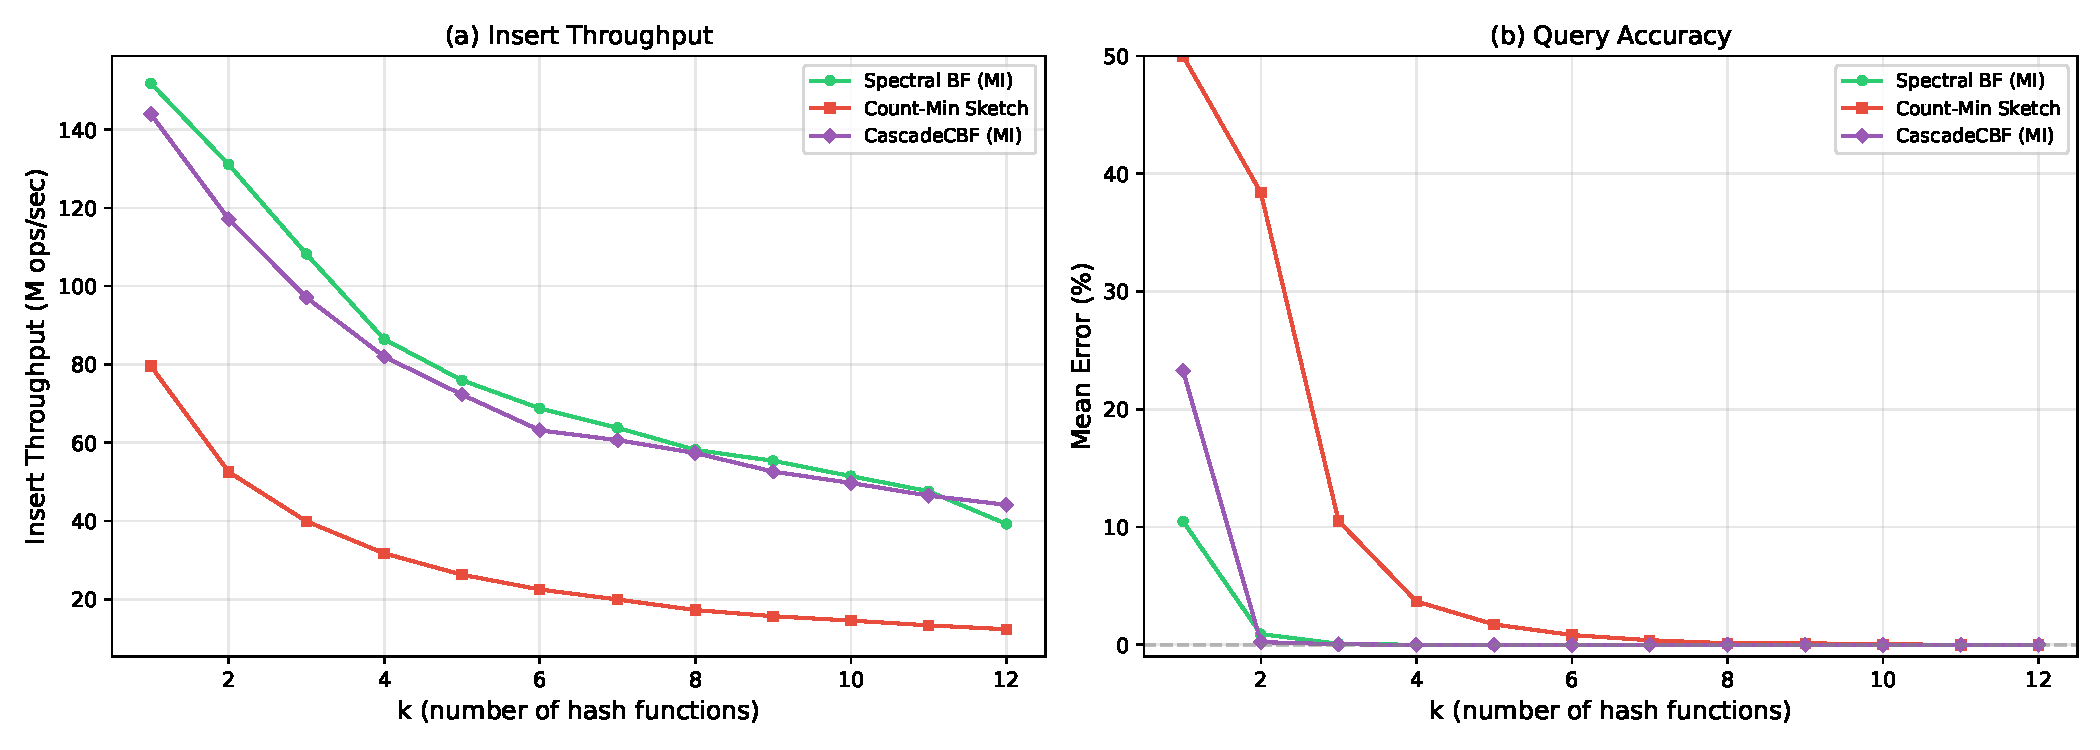
\includegraphics[width=8.2cm]{figures/k_sensitivity_combined.pdf}
  \caption{K-parameter sensitivity ($\alpha=1.5$): (a) throughput decreases with $k$; (b) error approaches 0\% as $k$ increases. CascadeCBF achieves 0\% error at $k \geq 4$.}
  \label{fig:k_sensitivity}
\end{figure}

Figure~\ref{fig:k_sensitivity} shows that \textbf{CascadeCBF achieves 0\% error at $k \geq 4$}, matching SBF-MI, while CMS requires $k \geq 11$. This difference arises because CMS uses separate counter arrays per hash function (requiring more hashes to achieve the same coverage), whereas CascadeCBF and SBF share a single counter array across all $k$ positions. The optimal $k^* \approx 0.693(m/n) \approx 4$ for our configuration explains why $k = 4$ suffices. Standard mode CascadeCBF provides 1.5--2$\times$ higher throughput than SBF-MI due to simpler increment logic; with minimal increment mode, throughput is comparable but accuracy improves for low-$k$ configurations.

\begin{figure}[ht]
  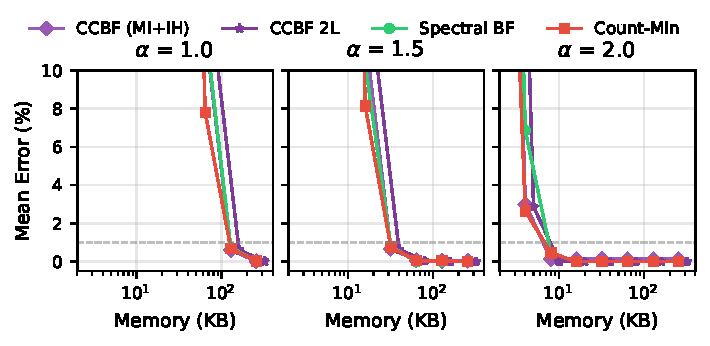
\includegraphics[width=8.2cm]{figures/memory_efficiency.pdf}
  \caption{Memory efficiency across Zipfian skew levels ($\alpha$). Single-layer CascadeCBF (MI+IH) matches SBF-MI and CMS accuracy. Two-layer version achieves exact counts at high skew.}
  \label{fig:memory}
\end{figure}

Figure~\ref{fig:memory} shows error vs. memory across Zipfian distributions. Single-layer CascadeCBF with minimal increment and independent hashes (MI+IH) matches the memory efficiency of SBF-MI and CMS: at $\alpha=1.5$, all achieve $<$1\% error with 32~KB. Two-layer CascadeCBF achieves 0\% error at higher skew ($\alpha=2.0$) with just 10~KB by cascading overflow to a second layer. This is particularly relevant for geospatial data, where population centers create extreme hotspots (e.g., $\alpha > 1.5$) that would overflow single-layer counters.

\subsection{Real-World Spatial Datasets}

We evaluate on two real geospatial datasets: \textbf{GDELT} (1.9M global news events with coordinates) and \textbf{COVID-19} (1.8M case locations sampled from 182M total). Table~\ref{tab:datasets} shows performance at 8192$\times$8192 rasterization with $k=8$.

\begin{table}[ht]
\centering
\caption{Performance on real geospatial datasets.}
\label{tab:datasets}
\small
\begin{tabular}{lccc}
\hline
\textbf{Implementation} & \textbf{Memory} & \textbf{GDELT} & \textbf{COVID-19} \\
 & (KB) & (s) & (s) \\
\hline
Spectral BF (MI) & 128 & 0.16 & 7.6 \\
Count-Min Sketch & 89 & 0.19 & 10.8 \\
CascadeCBF (MI) & 144 & 0.18 & 9.2 \\
CascadeCBF (std) & 144 & 0.13 & 7.0 \\
\hline
\end{tabular}
\end{table}

CascadeCBF in standard mode achieves the fastest insert times on both datasets, while MI mode provides comparable performance to alternatives. The COVID-19 dataset (higher skew due to population hotspots) shows greater variation across implementations, with CascadeCBF's multi-layer design efficiently handling the skewed distribution. Query times are comparable across all implementations ($\sim$0.27~ms per query).


%% =============================================================================
%% CONCLUSIONS
%% =============================================================================
\section{Conclusions}
\label{sec:conclusions}

CascadeCBF provides efficient cardinality estimation for power-law spatial data through cascading overflow between layers. The overflow bit protocol enables compact storage while maintaining cache locality---most operations touch only Layer~0. With minimal increment mode, CascadeCBF achieves 0\% error at $k \geq 4$, matching Spectral Bloom Filters while supporting counts up to $2^{31}$.

Evaluation on synthetic Zipfian data and real geospatial datasets (GDELT, COVID-19) confirms competitive performance: CascadeCBF matches or exceeds the insert throughput of alternatives while providing the flexibility of multi-layer overflow for highly skewed distributions. The multi-layer design enables exact counts at high skew levels where single-layer approaches accumulate errors.

Future work includes multiresolution re-randomization to restore hash uniformity across layers, deletion support via decrement operations, and GPU-accelerated implementations for streaming spatial analytics.


%% =============================================================================
%% DATA AND SOFTWARE AVAILABILITY
%% =============================================================================
\subsection*{Data and Software Availability}

The implementation of CascadeCBF is available as a header-only C++ library at \url{https://github.com/mlaass/counting-globimaps}. GDELT event data is publicly available from the GDELT Project (\url{https://www.gdeltproject.org}). COVID-19 case data was derived from the Johns Hopkins CSSE repository.


%% =============================================================================
%% DECLARATION OF GENERATIVE AI
%% =============================================================================
\subsection*{Declaration of Generative AI in writing}

The authors declare that they have used Generative AI tools in the preparation of this manuscript for language editing and improving sentence structure, but not for generating scientific content, research data, or substantive conclusions.


%% =============================================================================
%% ACKNOWLEDGEMENTS
%% =============================================================================
%\subsection*{Acknowledgements}
% TODO: Add acknowledgements if needed


%% =============================================================================
%% REFERENCES
%% =============================================================================
\bibliographystyle{copernicus-agile}
\bibliography{references}

\end{document}
